\documentclass{standalone}
\usepackage{tikz}
\usetikzlibrary{patterns, positioning}
\usepackage[sfdefault]{ClearSans} %% option 'sfdefault' activates Clear Sans as the default text font
\usepackage[T1]{fontenc}

\begin{document}
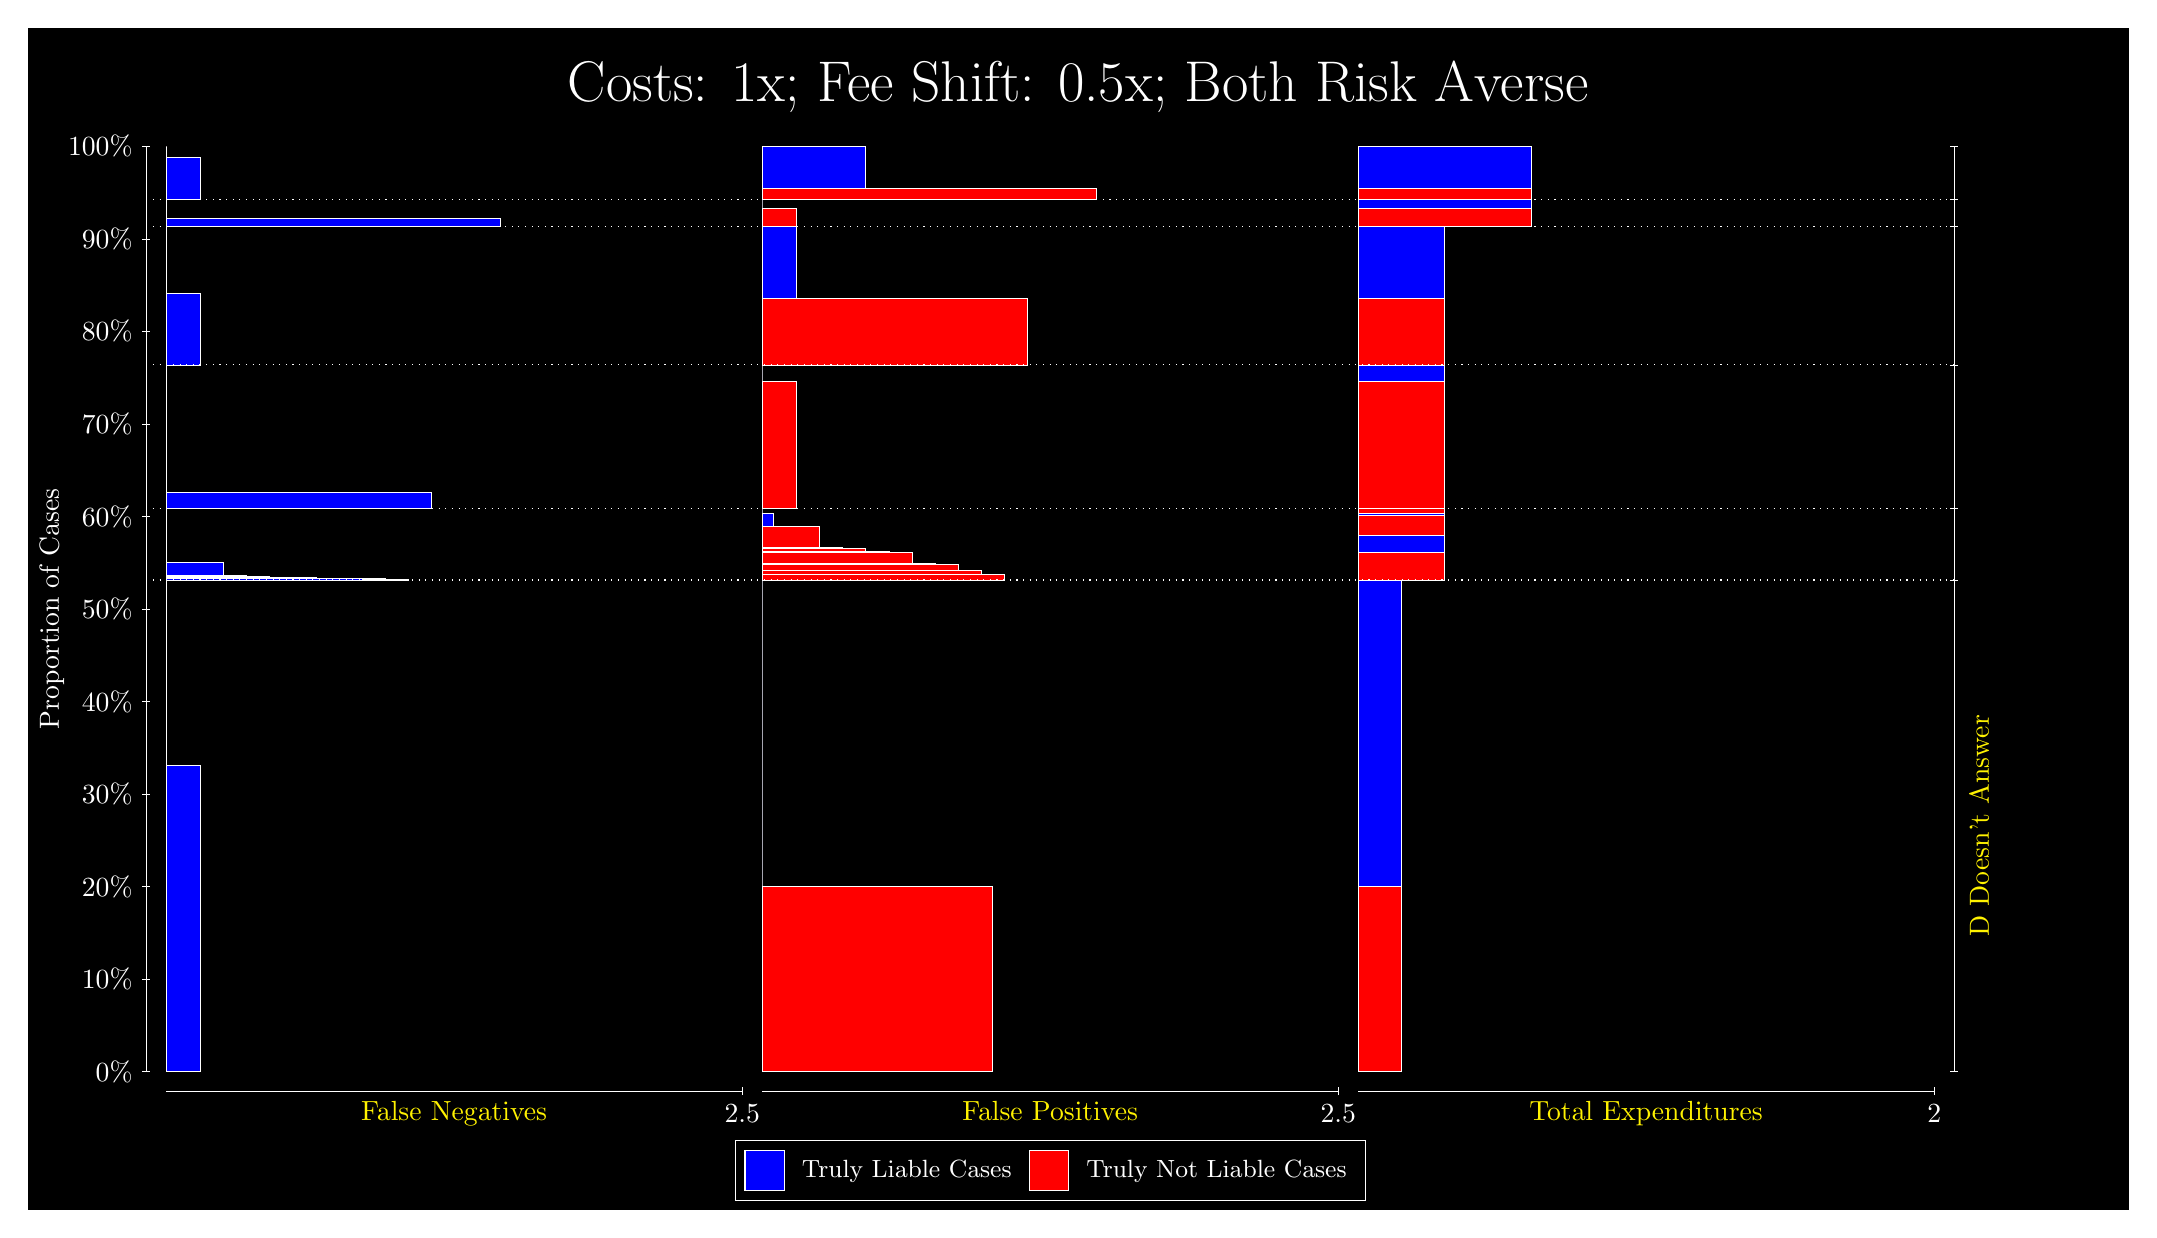
\begin{tikzpicture}
\draw[fill=black] (0,0) rectangle (26.667,15);
\draw[text=white] (0,13.5) rectangle (26.667,15) node[midway] {\huge Costs: 1x; Fee Shift: 0.5x; Both Risk Averse};
\draw[white, very thin] (1.5,1.75) -- (1.5,13.5);
\node[rotate=90, text=white, anchor=center] at (0.3, 7.625) {Proportion of Cases};
\draw[white, very thin] (1.45,1.75) -- (1.55,1.75);
\node[text=white, anchor=east] at (1.45, 1.75) {0\%};
\draw[white, very thin] (1.45,2.925) -- (1.55,2.925);
\node[text=white, anchor=east] at (1.45, 2.925) {10\%};
\draw[white, very thin] (1.45,4.1) -- (1.55,4.1);
\node[text=white, anchor=east] at (1.45, 4.1) {20\%};
\draw[white, very thin] (1.45,5.275) -- (1.55,5.275);
\node[text=white, anchor=east] at (1.45, 5.275) {30\%};
\draw[white, very thin] (1.45,6.45) -- (1.55,6.45);
\node[text=white, anchor=east] at (1.45, 6.45) {40\%};
\draw[white, very thin] (1.45,7.625) -- (1.55,7.625);
\node[text=white, anchor=east] at (1.45, 7.625) {50\%};
\draw[white, very thin] (1.45,8.8) -- (1.55,8.8);
\node[text=white, anchor=east] at (1.45, 8.8) {60\%};
\draw[white, very thin] (1.45,9.975) -- (1.55,9.975);
\node[text=white, anchor=east] at (1.45, 9.975) {70\%};
\draw[white, very thin] (1.45,11.15) -- (1.55,11.15);
\node[text=white, anchor=east] at (1.45, 11.15) {80\%};
\draw[white, very thin] (1.45,12.325) -- (1.55,12.325);
\node[text=white, anchor=east] at (1.45, 12.325) {90\%};
\draw[white, very thin] (1.45,13.5) -- (1.55,13.5);
\node[text=white, anchor=east] at (1.45, 13.5) {100\%};

\draw[white, very thin] (24.457,1.75) -- (24.457,13.5);
\draw[white, very thin] (24.407,1.75) -- (24.507,1.75);
\node[anchor=west] at (24.407, 1.75) {};
\draw[white, very thin] (24.407,7.9922) -- (24.507,7.9922);
\node[anchor=west] at (24.407, 7.9922) {};
\draw[white, very thin] (24.407,8.9046) -- (24.507,8.9046);
\node[anchor=west] at (24.407, 8.9046) {};
\draw[white, very thin] (24.407,10.725) -- (24.507,10.725);
\node[anchor=west] at (24.407, 10.725) {};
\draw[white, very thin] (24.407,12.483) -- (24.507,12.483);
\node[anchor=west] at (24.407, 12.483) {};
\draw[white, very thin] (24.407,12.826) -- (24.507,12.826);
\node[anchor=west] at (24.407, 12.826) {};
\draw[white, very thin] (24.407,13.5) -- (24.507,13.5);
\node[anchor=west] at (24.407, 13.5) {};

\draw[white, very thin, fill=blue] (1.75,1.75) rectangle (2.1891,5.6387);
\draw[white, very thin, fill=red] (1.75,5.6387) rectangle (1.75,7.9922);
\draw[white, very thin, fill=blue] (1.75,7.9922) rectangle (4.8239,8.0076);
\draw[white, very thin, fill=blue] (1.75,8.0076) rectangle (4.5312,8.0084);
\draw[white, very thin, fill=blue] (1.75,8.0084) rectangle (4.2384,8.0112);
\draw[white, very thin, fill=blue] (1.75,8.0112) rectangle (3.9457,8.0119);
\draw[white, very thin, fill=blue] (1.75,8.0119) rectangle (3.6529,8.0298);
\draw[white, very thin, fill=blue] (1.75,8.0298) rectangle (3.3602,8.0329);
\draw[white, very thin, fill=blue] (1.75,8.0329) rectangle (3.0674,8.0437);
\draw[white, very thin, fill=blue] (1.75,8.0437) rectangle (2.7746,8.0531);
\draw[white, very thin, fill=blue] (1.75,8.0531) rectangle (2.4819,8.2189);
\draw[white, very thin, fill=red] (1.75,8.2189) rectangle (1.75,8.9046);
\draw[white, very thin, fill=blue] (1.75,8.9046) rectangle (5.1167,9.1104);
\draw[white, very thin, fill=red] (1.75,9.1104) rectangle (1.75,10.725);
\draw[white, very thin, fill=blue] (1.75,10.725) rectangle (2.1891,11.638);
\draw[white, very thin, fill=red] (1.75,11.638) rectangle (1.75,12.483);
\draw[white, very thin, fill=blue] (1.75,12.483) rectangle (5.9949,12.592);
\draw[white, very thin, fill=red] (1.75,12.592) rectangle (1.75,12.826);
\draw[white, very thin, fill=blue] (1.75,12.826) rectangle (2.1891,13.357);
\draw[white, very thin, fill=red] (1.75,13.357) rectangle (1.75,13.5);
\draw[white, very thin, fill=red] (9.3189,1.75) rectangle (12.246,4.1035);
\draw[white, very thin, fill=blue] (9.3189,4.1035) rectangle (9.3189,7.9922);
\draw[white, very thin, fill=red] (9.3189,7.9922) rectangle (12.393,8.0616);
\draw[white, very thin, fill=red] (9.3189,8.0616) rectangle (12.1,8.1203);
\draw[white, very thin, fill=red] (9.3189,8.1203) rectangle (11.807,8.1888);
\draw[white, very thin, fill=red] (9.3189,8.1888) rectangle (11.515,8.2087);
\draw[white, very thin, fill=red] (9.3189,8.2087) rectangle (11.222,8.3449);
\draw[white, very thin, fill=red] (9.3189,8.3449) rectangle (10.929,8.3483);
\draw[white, very thin, fill=red] (9.3189,8.3483) rectangle (10.929,8.3549);
\draw[white, very thin, fill=red] (9.3189,8.3549) rectangle (10.636,8.4009);
\draw[white, very thin, fill=red] (9.3189,8.4009) rectangle (10.344,8.414);
\draw[white, very thin, fill=red] (9.3189,8.414) rectangle (10.051,8.6779);
\draw[white, very thin, fill=blue] (9.3189,8.6779) rectangle (9.4652,8.8437);
\draw[white, very thin, fill=blue] (9.3189,8.8437) rectangle (9.3189,8.9046);
\draw[white, very thin, fill=red] (9.3189,8.9046) rectangle (9.758,10.519);
\draw[white, very thin, fill=blue] (9.3189,10.519) rectangle (9.3189,10.725);
\draw[white, very thin, fill=red] (9.3189,10.725) rectangle (12.686,11.57);
\draw[white, very thin, fill=blue] (9.3189,11.57) rectangle (9.758,12.483);
\draw[white, very thin, fill=red] (9.3189,12.483) rectangle (9.758,12.717);
\draw[white, very thin, fill=blue] (9.3189,12.717) rectangle (9.3189,12.826);
\draw[white, very thin, fill=red] (9.3189,12.826) rectangle (13.564,12.969);
\draw[white, very thin, fill=blue] (9.3189,12.969) rectangle (10.636,13.5);
\draw[white, very thin, fill=red] (16.888,1.75) rectangle (17.437,4.1035);
\draw[white, very thin, fill=blue] (16.888,4.1035) rectangle (17.437,7.9922);
\draw[white, very thin, fill=red] (16.888,7.9922) rectangle (17.986,8.3483);
\draw[white, very thin, fill=blue] (16.888,8.3483) rectangle (17.986,8.5556);
\draw[white, very thin, fill=red] (16.888,8.5556) rectangle (17.986,8.8195);
\draw[white, very thin, fill=blue] (16.888,8.8195) rectangle (17.986,8.8349);
\draw[white, very thin, fill=red] (16.888,8.8349) rectangle (17.986,8.9005);
\draw[white, very thin, fill=blue] (16.888,8.9005) rectangle (17.986,8.9046);
\draw[white, very thin, fill=red] (16.888,8.9046) rectangle (17.986,10.519);
\draw[white, very thin, fill=blue] (16.888,10.519) rectangle (17.986,10.725);
\draw[white, very thin, fill=red] (16.888,10.725) rectangle (17.986,11.57);
\draw[white, very thin, fill=blue] (16.888,11.57) rectangle (17.986,12.483);
\draw[white, very thin, fill=red] (16.888,12.483) rectangle (19.083,12.717);
\draw[white, very thin, fill=blue] (16.888,12.717) rectangle (19.083,12.826);
\draw[white, very thin, fill=red] (16.888,12.826) rectangle (19.083,12.969);
\draw[white, very thin, fill=blue] (16.888,12.969) rectangle (19.083,13.5);
\draw[white, dotted] (1.5,7.9922) -- (24.457,7.9922);
\draw[white, dotted] (1.5,8.9046) -- (24.457,8.9046);
\draw[white, dotted] (1.5,10.725) -- (24.457,10.725);
\draw[white, dotted] (1.5,12.483) -- (24.457,12.483);
\draw[white, dotted] (1.5,12.826) -- (24.457,12.826);
\draw[white, very thin] (1.75,1.5) -- (9.0689,1.5);
\node[text=yellow, anchor=north] at (5.4094, 1.5) {False Negatives};
\draw[white, very thin] (9.0689,1.45) -- (9.0689,1.55);
\node[text=white, anchor=north] at (9.0689, 1.45) {2.5};

\draw[white, very thin] (9.3189,1.5) -- (16.638,1.5);
\node[text=yellow, anchor=north] at (12.978, 1.5) {False Positives};
\draw[white, very thin] (16.638,1.45) -- (16.638,1.55);
\node[text=white, anchor=north] at (16.638, 1.45) {2.5};

\draw[white, very thin] (16.888,1.5) -- (24.207,1.5);
\node[text=yellow, anchor=north] at (20.547, 1.5) {Total Expenditures};
\draw[white, very thin] (24.207,1.45) -- (24.207,1.55);
\node[text=white, anchor=north] at (24.207, 1.45) {2};

\node[text=yellow, centered, rotate=90] at (24.777, 4.8711) {D Doesn't Answer};






\draw (12.978300999999998,1.5) node[draw=none] (baseCoordinate) {};
\begin{scope}[align=center]
        \matrix[scale=0.5, draw=white, below=0.5cm of baseCoordinate, nodes={draw}, column sep=0.1cm]{
            \node[rectangle, draw, minimum width=0.5cm, minimum height=0.5cm, fill=blue] {}; &
            \node[draw=none, font=\small, text=white] (B) {Truly Liable Cases}; &
            \node[rectangle, draw, minimum width=0.5cm, minimum height=0.5cm, fill=red] {}; &
            \node[draw=none, font=\small, text=white] (B) {Truly Not Liable Cases}; \\
            };
\end{scope}

\end{tikzpicture}
\end{document}